%%%%::::::::::::::::::::::::::::::engineeringThesis V2::::::::::::::::::::::::::::::%%%
%%%::::::::::::::::::::::::::::::engineeringThesis V1::::::::::::::::::::::::::::::%%%
%%%:::::::::::::::::::::::::::::::::::::::::::::::::::::::::::::::::::::::::::::::
% Hello!!! Welcome to the \LaTeX{} template for your University of Malta, Faculty of Engineering thesis. This template was created (hacked!) by Alison Baldacchino B.Eng. (Hons) (2014)
%%%:::::::::::::::::::::::::::::::::::::::::::::::::::::::::::::::::::::::::::::::
% This is the preamble code required for part of the thesis type-setting. This
% code must be included before the \begin{document} in the engineeringThesis.tex file.
% To do this use the command \input{Preamble.tex}.
%%%:::::::::::::::::::::::::::::::::::::::::::::::::::::::::::::::::::::::::::::::
\documentclass[12pt,a4paper]{report}

\usepackage{packages/engineeringThesis}% Needed for further type-settings and commands
\usepackage{verbatim} % needed for the ''code" and other environments
\usepackage{amsfonts}
\usepackage{amsmath}
\usepackage{amssymb}
\usepackage{amsthm}
\usepackage{bibunits}% needed for the bibliography section
\usepackage{lipsum}% needed for the generating text in the example
\usepackage{booktabs}
\usepackage{svg}
\usepackage[binary-units=true]{siunitx}
\usepackage{float}
\usepackage{url}
\usepackage{multicol}
\usepackage{appendix}
\usepackage{color}
\usepackage{pdflscape}
\usepackage{pdfpages}
\usepackage{fancyvrb}
\usepackage{multirow} 
\usepackage[version=3]{mhchem}% usage \ce{CO2}, \ce{2H2 + O2 -> 2H2O} etc.

% BLOCK DIAGRAMS
\usepackage{tikz} % for flowcharts, and block diagrams

%%%:::::::::::::::::::::::::::::::::::::::::::::::::::::::::::::::::::::::::::::::
% The following environments are useful to present proofs in your thesis. These
% packages are not really necessary, if you don't need the code and proofs
% environments, so if you like you can delete from here till ``the next comment".
% Note that there are some examples below which obviously won't work once you
% remove this part
%%%:::::::::::::::::::::::::::::::::::::::::::::::::::::::::::::::::::::::::::::::
\theoremstyle{definition}
\newtheorem{definition}{Definition}[section]
\theoremstyle{definition}%plain}
\newtheorem{example}{Example}[section]
\theoremstyle{definition}%remark}
\newtheorem{proposition}{Proposition}[section]
\theoremstyle{definition}%remark}
\newtheorem{lemma}{Lemma}[section]
\theoremstyle{definition}%remark}
\newtheorem{corollary}{Corollary}[section]
\theoremstyle{definition}%remark}
\newtheorem{theorem}{Theorem}[section]
%%%:::::::::::::::::::::::::::::::::::::::::::::::::::::::::::::::::::::::::::::::
% The next comment!
%%%:::::::::::::::::::::::::::::::::::::::::::::::::::::::::::::::::::::::::::::::

%%%:::::::::::::::::::::::::::::::::::::::::::::::::::::::::::::::::::::::::::::::
% This section customises the headers of chapters, headers and footers.
%%%:::::::::::::::::::::::::::::::::::::::::::::::::::::::::::::::::::::::::::::::
% Customising headers and footers.
%:::::::::::::::::::::::::::::::::::::::::::::::::::::::::::::::::::::::::::::::::
\usepackage{fancyhdr}
\pagestyle{fancy}
\rhead{}
\lhead{\nouppercase{\textsc{\leftmark}}}
\renewcommand{\headrulewidth}{1pt}
\makeatletter
\renewcommand{\chaptermark}[1]{\markboth{\small\textsc{\@chapapp}\ \thechapter:\ \sc{#1}}{}}
\makeatother
%:::::::::::::::::::::::::::::::::::::::::::::::::::::::::::::::::::::::::::::::::
% Customising chapter headings.
%:::::::::::::::::::::::::::::::::::::::::::::::::::::::::::::::::::::::::::::::::
\usepackage{sectsty}
\chapterfont{\large\sc\centering}
\chaptertitlefont{\sc\centering}
\subsubsectionfont{\centering}
%%%:::::::::::::::::::::::::::::::::::::::::::::::::::::::::::::::::::::::::::::::


%%%:::::::::::::::::::::::::::::::::::::::::::::::::::::::::::::::::::::::::::::::
% PDF hyper-linking (set colours to black for printing)
%%%:::::::::::::::::::::::::::::::::::::::::::::::::::::::::::::::::::::::::::::::
\usepackage[colorlinks]{hyperref}
%\usepackage[figure,table]{hypcap}
\hypersetup{
	bookmarksnumbered,
	pdfstartview={FitH},
	citecolor={black},
	linkcolor={black},
	urlcolor={black},
	pdfpagemode={UseOutlines}
}
%%%:::::::::::::::::::::::::::::::::::::::::::::::::::::::::::::::::::::::::::::::

% Acronyms and Glossaries
% \usepackage{acronym}
\usepackage[acronym]{glossaries} % make a separate list of acronyms
\makeglossaries
\newacronym{pv}{PV}{Photovoltaic}
\newacronym{uv}{UV}{ultraviolet}
\newacronym{dssc}{DSC}{dye-sensitized solar cell}
\newacronym{sc}{SC}{semiconductor}
\newacronym{tio2}{\ce{TiO2}}{titanium dioxide}
\newacronym{als}{ALS}{Amyotrophic Lateral Sclerosis}
\newacronym{eog}{EOG}{Electrooculography}

\setlength{\headheight}{15pt}

%%%:::::::::::::::::::::::::::::::::::::::::::::::::::::::::::::::::::::::::::::::
% Sets the document to be line separated paragraphs not indentation separated
% paragraphs. To change to an indentation with no line skip simply change
% \parindent 0cm --> \parindent 1.3cm & \parskip 2ex --> \parskip 0ex
%%%:::::::::::::::::::::::::::::::::::::::::::::::::::::::::::::::::::::::::::::::
\parindent 0cm
\parskip 2ex

%%%:::::::::::::::::::::::::::::::::::::::::::::::::::::::::::::::::::::::::::::::
% End of preamble
%%%:::::::::::::::::::::::::::::::::::::::::::::::::::::::::::::::::::::::::::::::

\setlength\parindent{0pt}

\usepackage{multicol}
\usepackage[margin=10pt,small,hang,labelfont=bf,up]{caption} % Custom captions under/above floats in tables or figures


\newcommand{\Abstract}[1]{\normalfont\bfseries\itshape{Abstract\/}: \normalfont{#1}}

\newcommand{\Keywords}[1]{\normalfont\bfseries\itshape{Keywords\/}: \normalfont{#1}}
	
%%% HEADERS & FOOTERS
\usepackage{lastpage}
\usepackage{fancyhdr} % Headers and footers
\pagestyle{fancy} % All pages have headers and footers
\renewcommand{\headrulewidth}{0pt} % remove line below header
\fancyhead{} % Blank out the default header
\fancyfoot{} % Blank out the default footer
\fancyhead[C]{\textit{Thesis title}} % Custom header text
\fancyfoot[R]{\textit{Page \thepage \ of \pageref{LastPage}}} 
%----------------------------------------------------------------------------------------

\usepackage[style=ieee,backend=bibtex]{biblatex}
\footnotesize{\bibliography{ref}}

\begin{document}

\maketitle
\thispagestyle{empty}


\setcounter{page}{1}
\thispagestyle{fancy} % All pages have headers and footers

%----------------------------------------------------------------------------------------
%	ABSTRACT
%----------------------------------------------------------------------------------------
\Abstract{Write your abstract within these curly brackets. To clear and skip lines you will have the use the double backslash command. The best educators are the ones that inspire their students. That inspiration comes from a passion that teachers have for the subject they're teaching. Most commonly, that person spent their lives studying that subject, and they bring an infectious enthusiasm to the audience. I think many people have that enthusiasm, but they are prevented from being teachers because they didn't go through the teacher mill. Now you have teachers who have been through the teacher mill, yet they have no capacity to inspire anyone at all. It's the inspired student that continues to learn on their own. That's what separates the real achievers in the world from those who pedal along, finishing assignments. - Neil deGrasse Tyson.}\\

\Keywords{Educators, Teachers, Assignments}

%----------------------------------------------------------------------------------------
%	ARTICLE CONTENTS
%----------------------------------------------------------------------------------------

\begin{multicols}{2} % Two-column layout throughout the main article text

\section{INTRODUCTION}

This template was generated according to the University of Malta, Faculty of Engineering guidelines \cite{guidelines}. In the following chapters some examples regarding the use of this template and other common commands are illustrated. Most of this and other information can be acquired for the \LaTeX{} wiki books\footnote{\url{http://en.wikibooks.org/wiki/LaTeX/}}.

\section{FIRST SECTION}
\label{sec:sec1}

\lipsum[2]

\subsection{FIRST SUBSECTION} 
\label{ssec:ssec1.1}

\lipsum[3]

\subsection{SECOND SUBSECTION}
\label{ssec:ssec1.2}

\lipsum[1]

\section{SECOND SECTION}

\lipsum[5]

\subsection{FIRST SUBSECTION}

\lipsum[2]

\subsection{SECOND SUBSECTION}

\lipsum[2]

\begin{figure}[H]
\centering
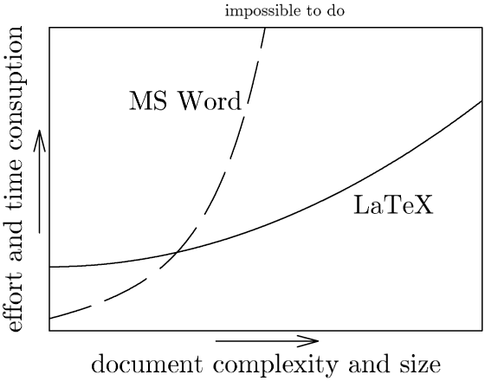
\includegraphics[width=0.45\textwidth]{pics/WordVsLatex}
\caption{WordVsLatex}
\label{fig:WordVsLatex}
\end{figure}

\section{RESULTS}

\lipsum[2]

\section{CONCLUSION}

\lipsum[2]

%----------------------------------------------------------------------------------------
%	REFERENCE LIST
%----------------------------------------------------------------------------------------

\printbibliography

%----------------------------------------------------------------------------------------

\end{multicols}

\end{document}
